\documentclass[10pt,conference]{IEEEtran}
\usepackage{graphicx}
\usepackage{listings}
\usepackage{color}

\lstset{
	basicstyle=\tiny,
	showstringspaces=false,
	%numbers=left,
	language=C,
	keywordstyle=\color{blue},
	frame=single
}

\begin{document}

\title{PID Control}

\author
{
 \IEEEauthorblockN{Matthew Lopez}
 \IEEEauthorblockA{Electrical Engineering Department, College of Engineering \\
 San Jose State University, San Jose, CA 94303 \\ 
 E-mail: matthew.lopez@sjsu.edu}
}

\maketitle

%
% Abstract
%
\begin{abstract}
This paper describes a methodology for developing and implementing a PID controller for the ARM 11 Processor. A positional error is read via the ADC, the data is ran through a PID controller, and the output is via the PWM of the ARM 11. Furthermore, the positional error is processed by a FFT to verify the data from the ADC is valid. The PID controller is shown to work when the positional error reaches a minimum.
\end{abstract}


%
% Introduction
%
\section{Introduction}
The purpose of this project is the develop and use a PID controller to ideally control a stepper motor. A stepper motor is not available, therefore the outputs are sent to a buzzer and LED. This project builds upon the previous two labs in that the GPIO ports are to be used and the ADC functionality is used.  In addition to the GPIO and ADC, the PWM feature of the ARM 11 is used as well.

\subsection{Tiny6410 and ARM11 Hardware}
The ARM family of processors is a significant player in the processor space. Nearly 95 percent of smartphones, tablets, and other portable devices use an ARM processor \cite{ARMSales}. The Tiny6410 Development board uses the ARM11 processor manufactured by Samsung. The Tiny6410 board exposes most of the capabilities and I/O features of the ARM11 processor in a format that is easy to use, i.e. USB or Ethernet ports, as well as a touchscreen. An overview of the ARM11 processor and it's I/O can be found in figure \ref{ARM11BlockDiagram}.

\begin{figure}[ht!]
	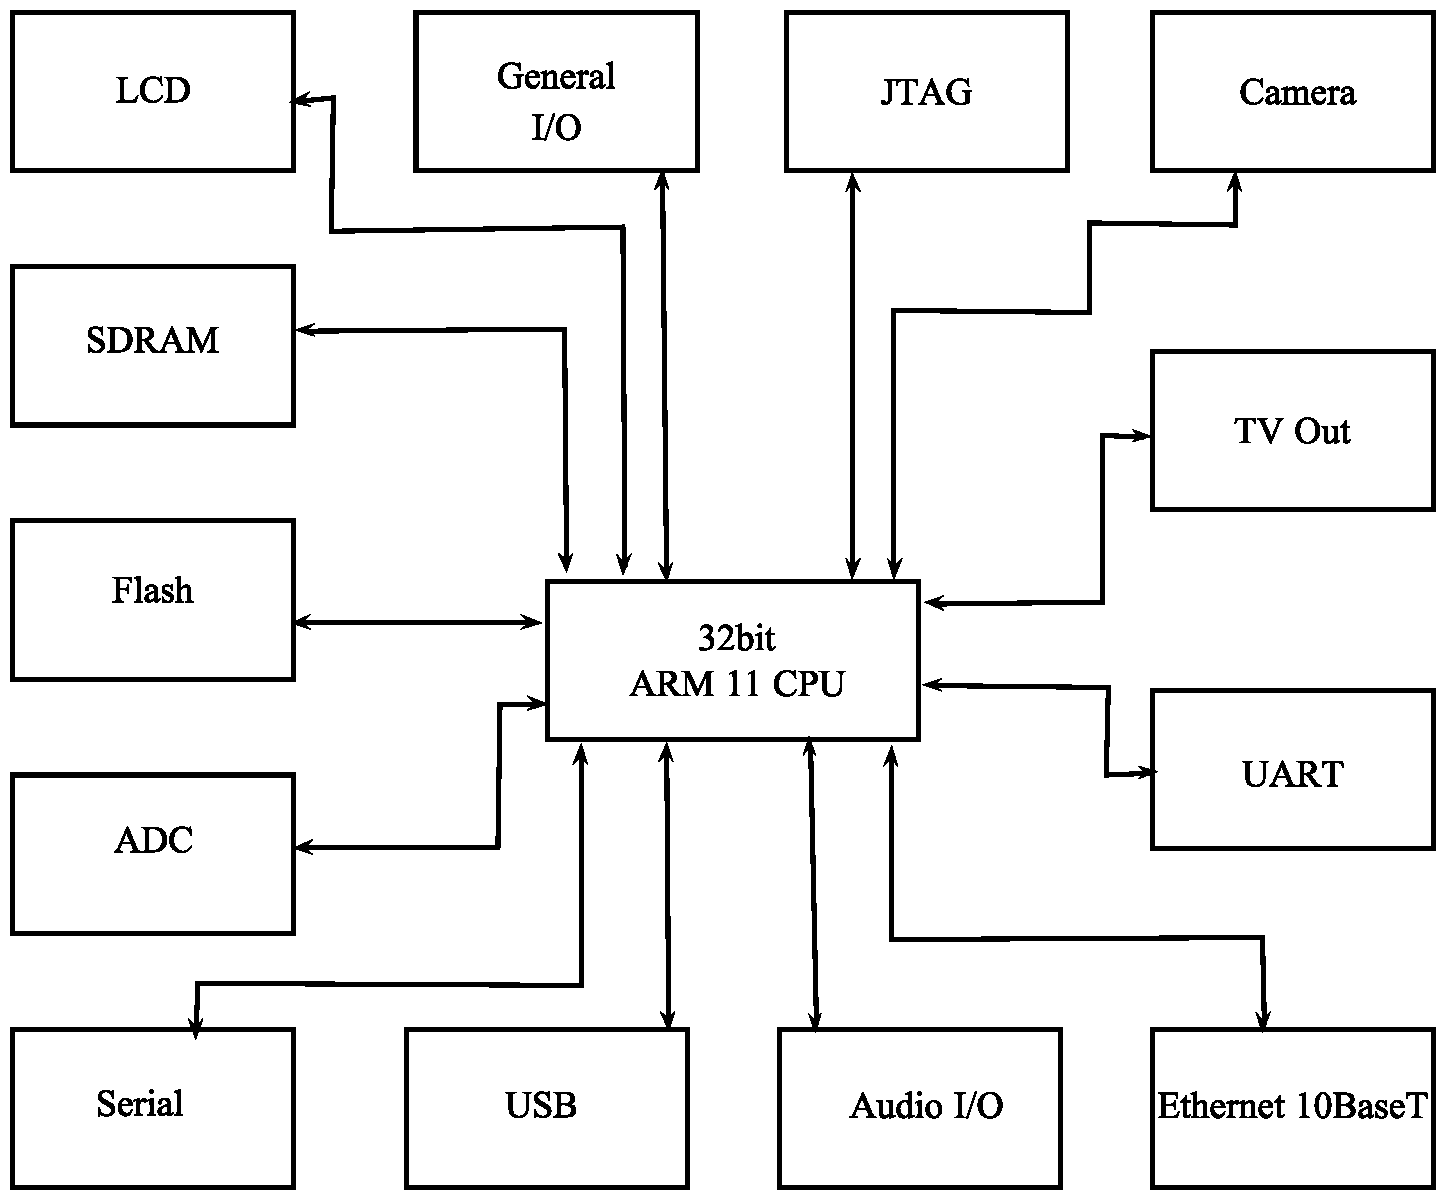
\includegraphics[scale=.30]{ARM11BlockDiagram}
	\caption{ARM11 and Tiny6410 I/O Block Diagram}\label{ARM11BlockDiagram}
\end{figure}


%
% Methodology
%
\section{Methodology}
This section will cover the objects and design of the hardware and the software. Since a stepper motor is not available, the features of the motor will be simulated with various hardware components.

\subsection{Control}
A PID controller is made up of three components,
\begin{enumerate}
	\item Proportional control. The proportional control attempts to correct the error in real time.
	\item Integral control. The integral control sums the error over time and attempts to control for excessive error.
	\item Derivative control The derivative control looks at the rate of change of error and attempts to correct large changes.
\end{enumerate}

A block diagram of the PID controller can be found at figure~\ref{F:PIDBlock}.

\begin{figure}[ht]
	\includegraphics[scale=0.3]{PIDBlock}
	\caption{Block Diagram}\label{F:PIDBlock}
\end{figure}

Together these three pieces compose the PID controller. The PID control takes as input the error from the requested command and the actual output. Each block in the PID controller has a gain, $K_p, K_i, K_d$ that is used to message the error values. Choosing correct values for the gains is an important part of control engineering. For this project the gains will not be determined and instead a different formula is used to find the outputs of the PID controller.
\[
	K_p = \frac{1}{3}\frac{e_0}{e_{max}}PWM_{max}
\]
where $e_0$ is the error for the current timeframe and $e_{max}$ is the maximum error and $PWM_{max}$ is the maximum output.
\[
	K_i = \frac{1}{3}\frac{\int e_0}{\int e_{max}}PWM_{max}
\]
where $\int e_0$ is the total error for the entire timeframe and $\int e_{max}$ is the maximum error and $PWM_{max}$ is the maximum output.
\[
	K_d = \frac{1}{3}\frac{De_0}{De_{max}}PWM_{max}
\]
where $De_0$ is the derivative error for the current timeframe and $De_{max}$ is the maximum derivative error and $PWM_{max}$ is the maximum output.

\subsection{Hardware}
There are several components that make up the hardware used for this project.

\subsubsection{ARM11}\label{ARM11HW}
The ARM 11 processor provides 4 ADC channels with resolution of 10 or 12 bits. The channel selection, bit resolution, and other controls are done via the ADCCON control register \cite{Samsung}. The converted data from the analog device is placed into one of two data registers, ACDDAT0 or ADCDAT1 \cite{Samsung}.

The Tiny6410 board provides an interface to only 2 of the 4 ADC channels. On connector CON1, Channel 2 on pin AIN2 and Channel 3 on pin AIN3 \cite{HWHandout}.

To control and use general I/O Port E, the ARM11 provides two registers. GPECON is the control register that is used to tell the ARM11 how the individual pins of Port E are to be used \cite{Samsung}. For this project the following pins are used,
\begin{enumerate}
	\item GPE1. Used for input; read the switch state. GPECON bits [3:0] are set to 0x0.
	\item GPE3. Used for output; turn on and off the LED. GPECON bits [15:12] are set to 0x1.
\end{enumerate}
The other pins, GPE0, GPE2, and GPE4 are not used and as a result the GPECON bits corresponding to these pins are set to 0x0. With all of this together the value 0x1000 is written to the GPECON register.

To read the input or to write an output, the register GPEDAT is used \cite{Samsung}.  Each bit in GPEDAT corresponds to one of the pins in Port E.  GPEDAT bit 0 is for pin GPE0, GPEDAT bit 1 is for GPE1, and so on. 

The Tiny6410 board provides the physical pins that correspond to the GPE I/O ports, labeled CON 1 \cite{HWHandout}. Unfortunately, GPE0 does not have a pin assigned to it, only GPE1 through GPE4.

The ARM 11 processor also provides 2 PWM outputs. Unfortunately, the Tiny6410 board does not provide direct access to the PWM pins. One of the PWM outputs is connected to a buzzer on the Tiny6410 board, so as the PWM is controlled, the buzzer will change pitch.

\subsubsection{Prototype Board}\label{ProtoBoard}
The prototype board is a board that is separate from the Tiny6410 board. For this project the hardware on the prototype board consists of,
\begin{enumerate}
	\item Pins to connect the prototype board with the Tiny6410 board.
	\item LEDs with a current limiting resistor.  These LEDs provide indication of requested speed and when the final position is reached.
	\item Several resistors to limit the input voltage and current into the ADC.
	\item A potentiometer to adjust the voltage into the ADC and as a result change the positional error.
	\item A 5VDC power supply sourced from a USB port \cite{USB5VDC}.
\end{enumerate}

\subsection{Stepper Motor}\label{SS:StepperMotor}
While this project doesn't use a stepper motor, the understanding of a stepper motor is advisable. An example motor is described in table~\ref{T:stepper_motor} \cite{StepperMotor}

\begin{table}[h]
\begin{tabular}{ | c | c | }
	\hline
	\textbf{Function} & \textbf{Value} \\ \hline
	Recommended Voltage & 5VDC \\ \hline
	Steps per Revolution Not including Gearbox & 1:8 \\ \hline
	Gearbox & 1:64 \\ \hline
	Steps per Revolution With Gearbox & 1:512 \\ \hline
	Step per Degree & 1.42 \\ \hline
	Weight & 37g \\ \hline
	Dimensions & 28mm diameter, 20mm tall not including 9mm shaft with 5mm diameter \\ \hline
\end{tabular}
\caption{Connections between Tiny6410 and Prototype Board}\label{T:stepper_motor}
\end{table}


\subsection{Software}\label{Software}
There are two software programs used for the project,
\begin{enumerate}
	\item The device driver.
	\item The user level program.
\end{enumerate}

\subsubsection{Device Driver}\label{DeviceDriver}
The device driver is the software that operates at the level of the Linux kernel and has direct access to the hardware. The device driver is broken up into several sections,
\begin{enumerate}
	\item Initialization. The control register is set to the default values. The driver is also registered with the Linux kernel and can now be found by user level programs.
	\item Clean up. Deregister the driver from the Linux kernel.
	\item I/O Control. The driver needs to provide a method for user level programs to interact with the hardware. The device driver therefore implements the \emph{ioctl} function. The user level control function will send commands to the driver's \emph{ioctl} function to perform some action and the function will return a status or data value. The function can interact with the GPECON and ADCCON registers first mentioned in section \ref{ARM11HW}. 
	\item Read. The device driver exposes a \emph{read} function that allows the user level program to read from the ADC. The read function can interact directly from the hardware, reading from the ADCDAT register and then copying the data into a buffer in user space.
\end{enumerate}


\subsubsection{User Level Program}
The user level program is the software that operates at the level that the user has access to.  Direct access to the hardware is not allowed. As mentioned in the device driver section \ref{DeviceDriver}, the user level program uses \emph{ioctl} and \emph{read} to interact with the device driver. The code is straightforward,
\begin{enumerate}
	\item The program translates the user into a command \emph{ioctl} from the device driver can understand. A common header file is shared between the user level program and the device driver to ensure the commands are consistent between the two programs.
	\item Call \emph{ioctl} with the appropriate command and read the results or error status.
	\item Call \emph{read} to read the data from the ADC.
\end{enumerate}


%
% Implementation
%
\section{Implementation}

\subsection{Hardware}
The data connection between the prototype board and the Tiny6410 board is a ribbon cable specific to the Tiny6410 board. Individual wires are exposed at the prototype board to facilitate the individual connections. The power supply for the ADC validation circuit is 5VDC USB supplied from the Tiny6410 board.  An overall block diagram of the setup can be found in figure \ref{BlockDiagram}. A schematic of the prototype board can be found in figure \ref{F:cmpe242_lab3}.

\begin{figure}[ht]
	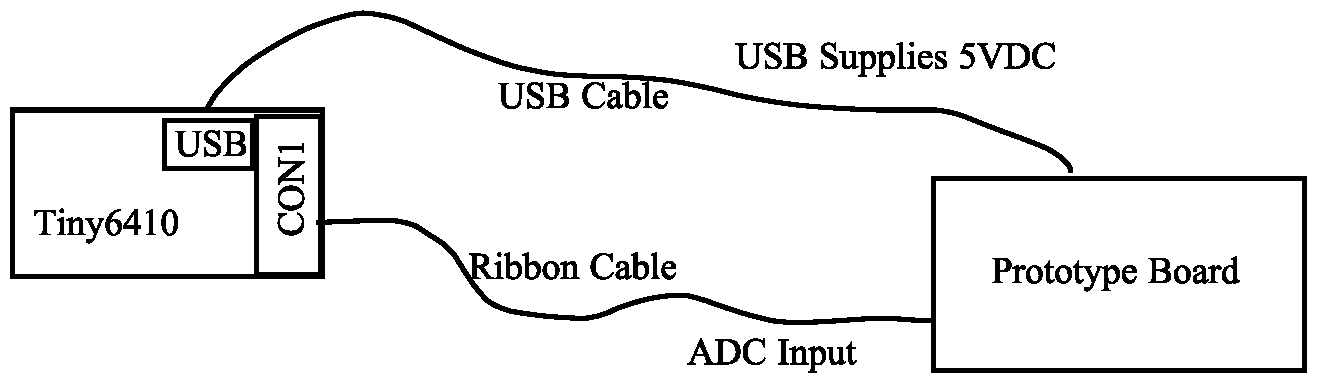
\includegraphics[scale=.35]{BlockDiagram}
	\caption{Block Diagram}\label{BlockDiagram}
\end{figure}

\begin{figure}[ht]
	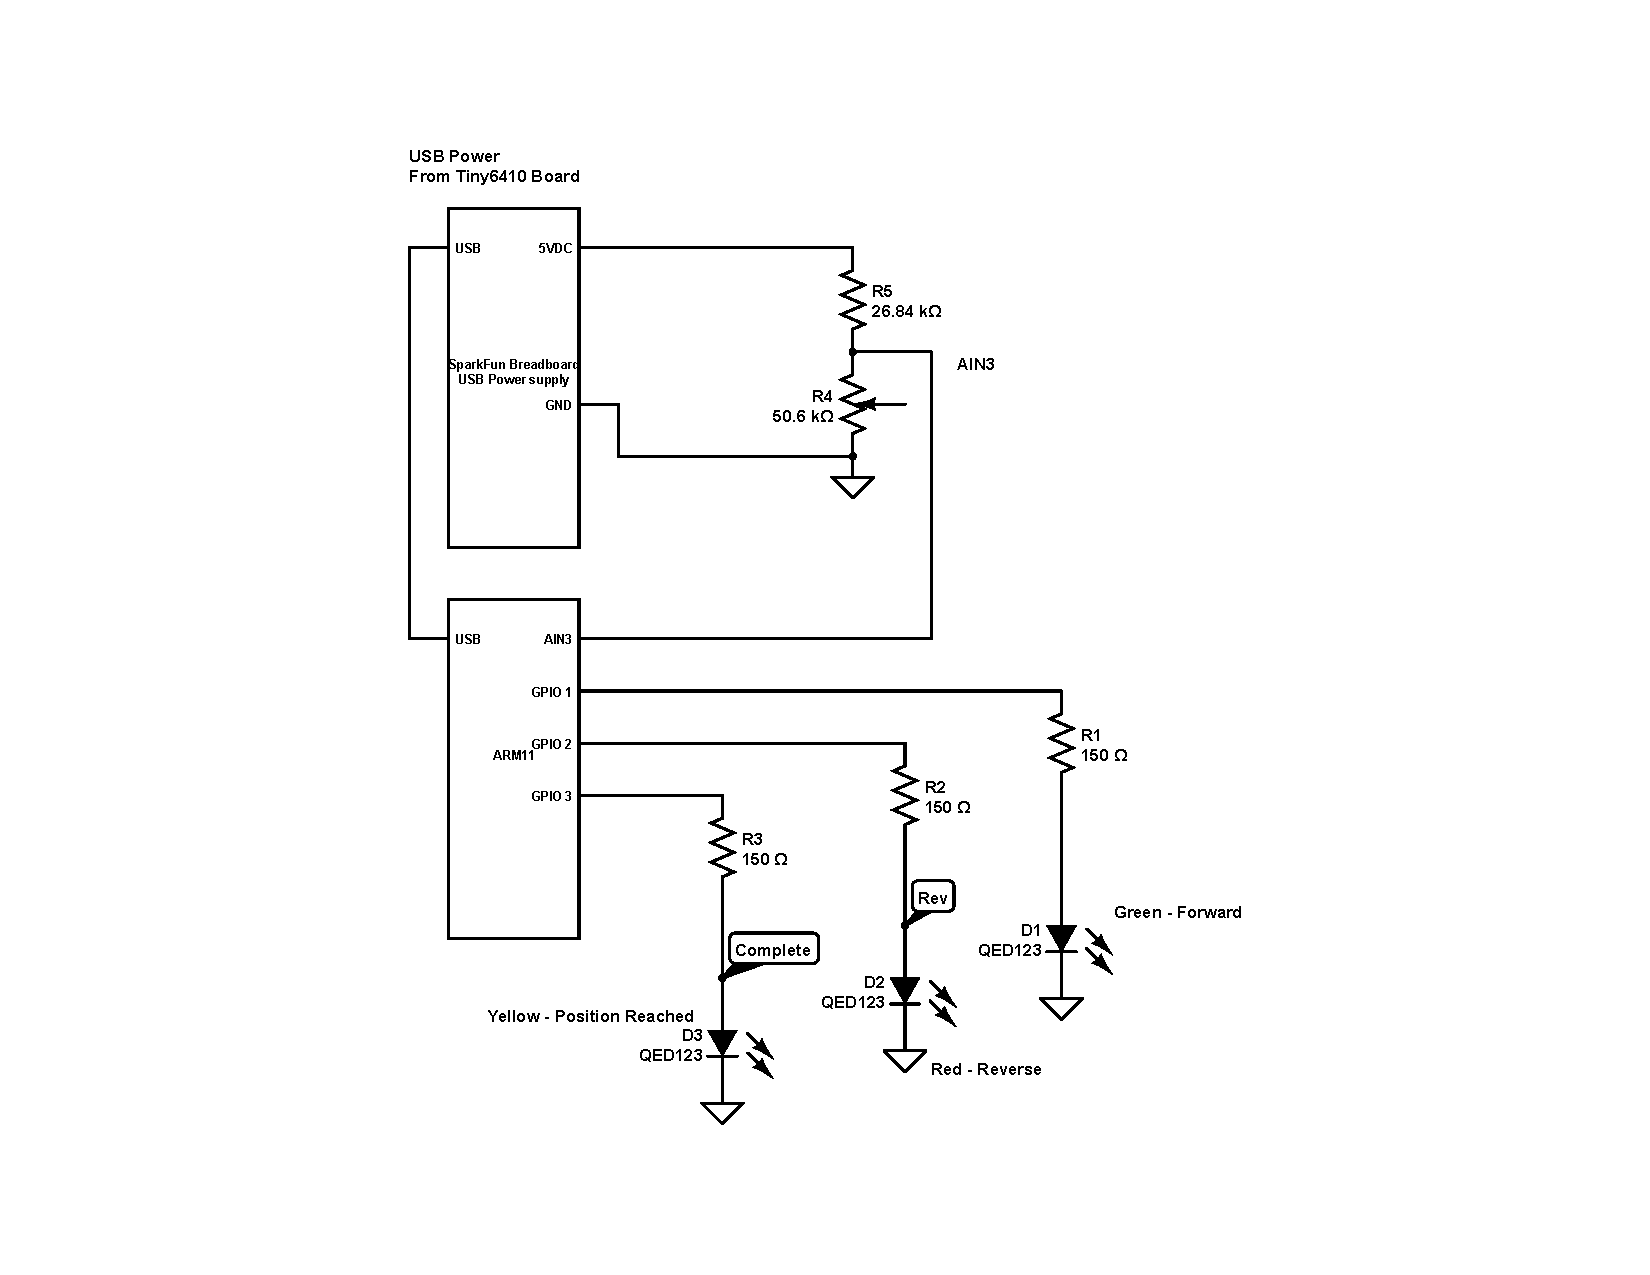
\includegraphics[scale=.45]{cmpe242_lab3}
	\caption{Schematic for Prototype Board}\label{F:cmpe242_lab3}
\end{figure}

A 5VDC power source was used to drive the ADC circuit with the potentiometer adjusting the positional error. Three LED's are used to indicate forward direction, backward direction, and position reached.

\subsection{Software}
The software will perform the following,
\begin{enumerate}
	\item Process user arguments. The user is required to select a position and a direction.
	\item Analyze the ADC.
	\item Get the error, run through PID, and get new values for PWM. Continue to do so until error is zero.
	\item Blink the 'complete led' for 3 seconds. Turn off everything.
\end{enumerate}
Pseudocode for the PID control can be found in listing~\ref{L:PIDcode}

\begin{figure}[ht]
	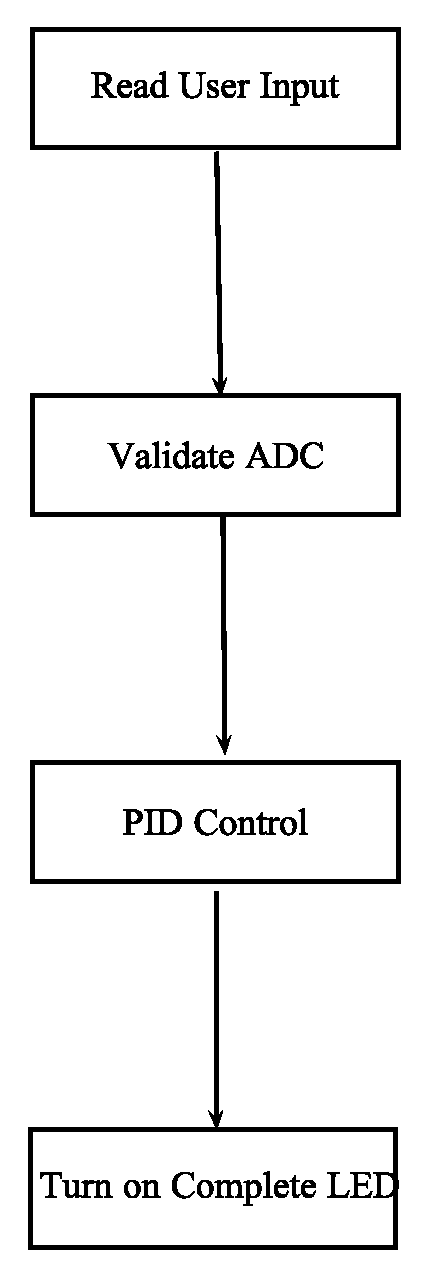
\includegraphics[scale=.45]{FlowChart}
	\caption{Flow Chart}\label{F:FlowChart}
\end{figure}

\begin{lstlisting}[language=C, frame=single, caption=Pseudo Code for PID Controller,label=L:PIDCode]
	do until motor reaches desired position
		error = read_adc()
		if error == 0
			then stop motor and return control to user
		else
			total_error = get_total_error() // integral of error
			error_slope = get_derivative_error() // derivative of the error
			Kp = (error)/(max_error)*1/3*MotorMax
			Ki = (total_error)/(max_total_error)*1/3*MotorMax
			Kd = (error_slope)/(max_slope_error)*1/3*MotorMax

			new_freq = Kp + Ki + Kd
			command_motor( new_freq )
		end if
	end do loop
\end{lstlisting}

%
% Testing and Verification
%
\section{Testing and Verification}
The user program was started with a desired position. The potentiometer was adjusted until the input voltage to the ADC was zero, thus simulating the error going to zero. As the error tends to zero, the frequency for the PWM decreases as well. Since the PWM is connected to the buzzer, there is a noticeable change in the pitch to the buzzer. Thus the PID controller works as expected.

The results from the FFT for validating the ADC were very good as nearly all of the power was at the zero frequency, which is what to be expected for DC values.
\begin{figure}[ht]
	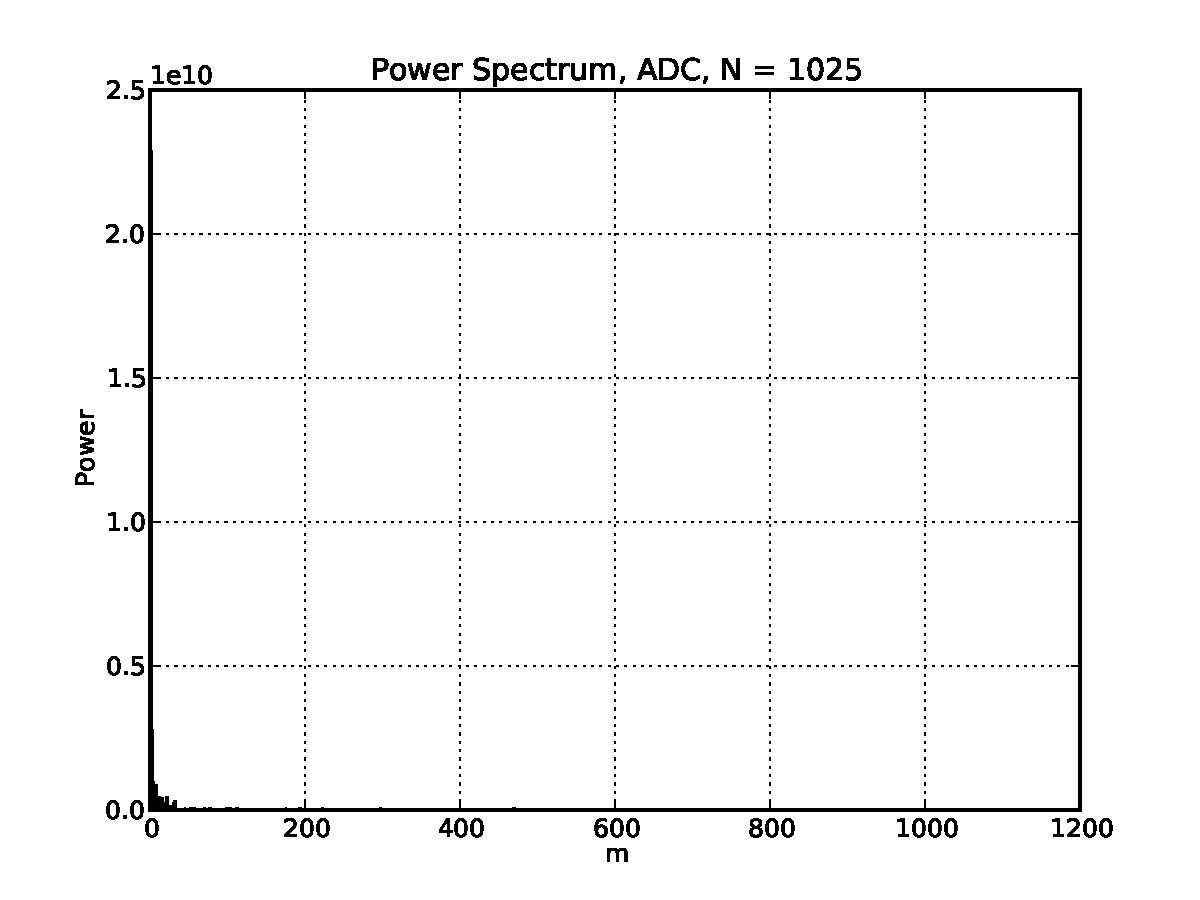
\includegraphics[scale=.50]{power_spectrum_adc_1025}
	\caption{Power Spectrum for ADC and N = 1025}\label{F:power_spectrum_adc_1025}
\end{figure}

%
% Conclusion
%
\section{Conclusion}
In conclusion, combining the previous two labs with PWM and PID control produces a fully functional embedded controller. The PID controller works to correct the error and the user program has shown the using techniques and code from the previous labs works as well.

%
% thebibliography
%
\begin{thebibliography}{9}
\bibitem{LDD}
Jonathan Corbet, Alessandro Rubini, and Greg Kroah-Hartman,
\emph{Linux Device Drivers, Third Edition},
O'Reilly Media,
Sebastopol, CA,
2005

\bibitem{Samsung}
-,
\emph{User's Manual \\ S3C6410X \\ RISC Microprocessor},
Samsung Electronics, Inc.,
2008

\bibitem{HWHandout}
Harry Li,
\emph{Handout On Hardware of the ARM11 Development Board},
Computer Engineering Department, College of Engineering,
 San Jose State University,
Spring, 2013

\bibitem{FFTHandout}
Harry Li,
\emph{Handout On The Fast Fourier Transform},
Computer Engineering Department, College of Engineering,
 San Jose State University,
Spring, 2013

\bibitem{USB5VDC}
- (31 Mar. 2013),
\emph{Breadboard Power Supply USB - 5V/3.3V.}
[Online]
Available: https://www.sparkfun.com/products/8376

\bibitem{ARMSales}
Agam Shah (Jan 22, 2013)
\emph{Processor market to get boost from smartphones, tablets}
[Online]
Available: http://www.pcworld.com/article/2025967/processor-market-to-get-boost-from-smartphones-tablets.html

\bibitem{FFTO}
- (March 23, 2013)
\emph{Fast Fourier transform}
[Online]
Available: https://en.wikipedia.org/wiki/Fast\_Fourier\_transform

\bibitem{StepperMotor}
- (May 6, 2013)
\emph{Small Reduction Stepper Motor - 5VDC 512 Step}
[Online]
Available: https://www.adafruit.com/products/858

\end{thebibliography}

\end{document}
